\hypertarget{ux56feux5f62ux754cux9762}{%
\subsection{图形界面}\label{ux56feux5f62ux754cux9762}}

Python 支持多种图形界面的第三方库,包括:

\begin{itemize}
\item
  Tk
\item
  wxWidgets
\item
  Qt
\item
  GTK
\end{itemize}

等等。

但是 Python 自带的库是支持 Tk 的 Tkinter,使用
Tkinter,无需安装任何包,就可以直接使用。本章简单介绍如何使用 Tkinter
进行 GUI 编程。

\hypertarget{tkinter}{%
\subsubsection{Tkinter}\label{tkinter}}

我们来梳理一下概念:

我们编写的 Python 代码会调用内置的 Tkinter,Tkinter 封装了访问 Tk
的接口;

Tk 是一个图形库,支持多个操作系统,使用 Tcl 语言开发;

Tk 会调用操作系统提供的本地 GUI 接口,完成最终的 GUI。

所以,我们的代码只需要调用 Tkinter 提供的接口就可以了。

\hypertarget{ux7b2cux4e00ux4e2a-gui-ux7a0bux5e8f}{%
\subsubsection{第一个 GUI
程序}\label{ux7b2cux4e00ux4e2a-gui-ux7a0bux5e8f}}

使用 Tkinter 十分简单,我们来编写一个 GUI 版本的 ``Hello, world!''。

第一步是导入 Tkinter 包的所有内容:

\begin{pythoncode}
from tkinter import *
\end{pythoncode}

第二步是从\texttt{Frame}派生一个\texttt{Application}类,这是所有 Widget
的父容器:

\begin{pythoncode}
class Application(Frame):
    def __init__(self, master=None):
        Frame.__init__(self, master)
        self.pack()
        self.createWidgets()

    def createWidgets(self):
        self.helloLabel = Label(self, text='Hello, world!')
        self.helloLabel.pack()
        self.quitButton = Button(self, text='Quit', command=self.quit)
        self.quitButton.pack()
\end{pythoncode}

在 GUI 中,每个 Button、Label、输入框等,都是一个 Widget。Frame
则是可以容纳其他 Widget 的 Widget,所有的 Widget 组合起来就是一棵树。

\texttt{pack()}方法把 Widget
加入到父容器中,并实现布局。\texttt{pack()}是最简单的布局,\texttt{grid()}可以实现更复杂的布局。

在\texttt{createWidgets()}方法中,我们创建一个\texttt{Label}和一个\texttt{Button},当
Button 被点击时,触发\texttt{self.quit()}使程序退出。

第三步,实例化\texttt{Application},并启动消息循环:

\begin{pythoncode}
app = Application()

app.master.title('Hello World')

app.mainloop()
\end{pythoncode}

GUI
程序的主线程负责监听来自操作系统的消息,并依次处理每一条消息。因此,如果消息处理非常耗时,就需要在新线程中处理。

运行这个 GUI 程序,可以看到下面的窗口:

 
 \begin{figure}[htp]
	\centering
	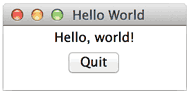
\includegraphics[width=0.6\linewidth]{fig/972676918012640.png}
\end{figure}


点击 ``Quit'' 按钮或者窗口的 ``x'' 结束程序。

\hypertarget{ux8f93ux5165ux6587ux672c}{%
\subsubsection{输入文本}\label{ux8f93ux5165ux6587ux672c}}

我们再对这个 GUI
程序改进一下,加入一个文本框,让用户可以输入文本,然后点按钮后,弹出消息对话框。

\begin{pythoncode}
from tkinter import *
import tkinter.messagebox as messagebox

class Application(Frame):
    def __init__(self, master=None):
        Frame.__init__(self, master)
        self.pack()
        self.createWidgets()

    def createWidgets(self):
        self.nameInput = Entry(self)
        self.nameInput.pack()
        self.alertButton = Button(self, text='Hello', command=self.hello)
        self.alertButton.pack()

    def hello(self):
        name = self.nameInput.get() or 'world'
        messagebox.showinfo('Message', 'Hello, %s' % name)

app = Application()

app.master.title('Hello World')

app.mainloop()
\end{pythoncode}

当用户点击按钮时,触发\texttt{hello()},通过\texttt{self.nameInput.get()}获得用户输入的文本后,使用\texttt{tkMessageBox.showinfo()}可以弹出消息对话框。

程序运行结果如下:

 
 \begin{figure}[htp]
	\centering
	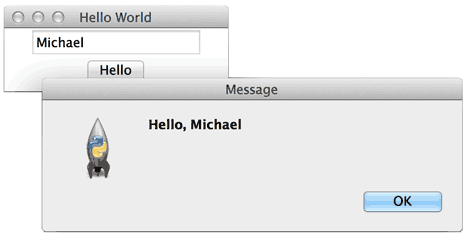
\includegraphics[width=0.6\linewidth]{fig/972677353581536.png}
\end{figure}


\hypertarget{ux5c0fux7ed3}{%
\subsubsection{小结}\label{ux5c0fux7ed3}}

Python 内置的 Tkinter 可以满足基本的 GUI 程序的要求,如果是非常复杂的
GUI 程序,建议用操作系统原生支持的语言和库来编写。

\hypertarget{ux53c2ux8003ux6e90ux7801}{%
\subsubsection{参考源码}\label{ux53c2ux8003ux6e90ux7801}}

\href{https://github.com/michaelliao/learn-python3/blob/master/samples/gui/hello_gui.py}{hello\_gui.py}

